\chapter{Introdução}
Arquitetura Orientada a Serviços, ou do inglês \textit{Service-Oriented Architecture} (SOA), tem surgido ao longo dos últimos anos como uma das abordagens preferidas para construção de sistemas~\cite{erl2008soa}. Com objetivos alinhados aos objetivos do paradigma SOC \textit{(Service-Oriented Computing)}, SOA possibilita a criação de novas aplicações com maior coerência, rapidez e diminuição nos custos, tudo isso com excelente aproveitamento do legado~\cite{erl2008soa}.

Baseada em padrões abertos e na visão onipresente da Internet, SOA tem como princípio fundamental a idéia de serviços como unidades que representam módulos do negócio ou funcionalidades da aplicação~\cite{erl2008soa}~\cite{imb2007soa}. Na visão de SOA, um serviço é um componente que implementa uma função de negócio. Ele pode responder a requisições ocultando os detalhes de sua implementação e é descrito através de contratos que expressam seu objetivo e suas capacidades. Buscando maior agilidade, flexibilidade e reuso de componentes pré-existentes no desenvolvimento de aplicações, diversas empresas de tecnologia da informação vêm adotando SOA na construção de seus sistemas.

Nesse contexto, temos a plataforma de serviços OSGi (\textit{Open Services Gateway initiative}~\cite{alliance2007osgi}. OSGi provê suporte à modelagem e desenvolvimento de sistemas modulares na linguagem Java~\cite{hall2010osgi}. A idéia básica é resolver o problema de criar softwares monolíticos, ou seja, softwares projetados sem modularidade, facilitando a reutilização e manutenção de  componentes, o que torna a solução mais robusta, barata e confiável~\cite{davis2009open}.

OSGi introduz um modelo de programação orientada a serviço, o que alguns autores apresentam como \textit{SOA in a Virtual Machine}~\cite{hall2010osgi}, separando de fato a interface da implementação. Isso mostra um grande potencial para a construção de aplicações orientadas à serviço.

Outra tecnologia que compartilha vários princípios de SOC é a tecnologia de \textit{Web Services}. \textit{Web Services} fornecem uma forma padrão de interoperabilidade entre diferentes aplicações, capaz de executar em uma variedade de plataformas e \textit{frameworks}~\cite{w3c2002ws}.

Assim, em uma arquitetura orientada a serviços, módulos podem consumir serviços providos por tecnologias diferentes, apenas identificando o serviço requerido e realizando o \textit{binding}. Estabelecendo assim um contrato entre o consumidor e o provedor do serviço~\cite{oracle2005ws}.

%//TODO: ORGANIZAR TRECHO
Esses contratos são especificados através de SLAs (\textit{Service Level Agreement}). Em um SLA temos basicamente uma descrição de um acordo entre o provedor e consumidor de um determinado serviço. Esse acordo define propriedades de como consumidor terá acesso ao serviço, geralmente essas estão relacionadas a atributos não-funcionais (\textit{e.g. reponse time}).

%//TODO: COLOCAR REFERENCIA PENALIDADE QUEBRA
Porém, uma tarefa complexa neste cenário é garantir que os acordos a nível de serviço, SLAs, entre o consumidor e provedor são realmente respeitados. Além disso, prevenir uma quebra de contrato, onde o provedor não cumpre com os requisitos não-funcionais definidos nos SLAs, é outro ponto complexo a ser atacado, pois, na maioria dos casos, quando é caracterizada uma quebra de contrato o provedor pode sofrer algum tipo de penalidade, ou mesmo, perder um potencial consumidor de seus serviços.

Deste modo, o monitoramento dos serviços aliado à análise dos dados monitorados, surge como uma possível solução para o problema de garantir o cumprimento dos contratos entre provedores e consumidores de serviços. Ainda mais, o resultado dessa análise aliada a um mecanismo de auto-gerenciamento do ambiente onde estes serviços são executados, surge como uma alternativa viável à manutenção dos contratos por parte dos provedores. Uma vez que, na definição dos SLAs, o provedor apresenta suas capacidades funcionais e não-funcionais (atributos de QoS), e os consumidores ao buscarem serviços, definem contratos com base nessas informações dispobibilizadas por esses provedores, comprovando as necessidades citadas acima.

\section{Objetivos}

\begin{figure}[htp]
\centering
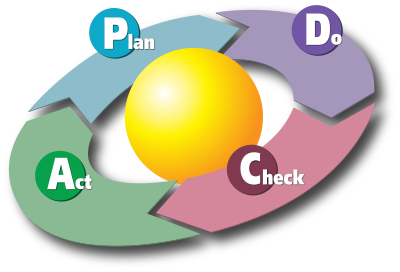
\includegraphics[width=5cm]{chapters/intro/pdca_cycle.png}
\caption[Ciclo PDCA]{Ciclo PDCA de Desenvolvimento com Foco na Melhoria Contínua.}
\end{figure}
